%%%%%%%%%%%%%%%%%%%%%%%%%%%%%%%%%%%%%%%%%%%%%%%%%%%%%%%%%%%
% Capitolo 6

\chapter{Realizzazione del progetto}
\label{progetto}

In questo capitolo verrà discussa l'effettiva realizzazione del progetto, ovvero analisi dei requisiti, progettazione, sviluppo e testing, secondo le metodologie agili.
Ogni progetto inizia con la stesura di un \textit{Project Charter} (Documento di inizio progetto), che, non essendo di interesse in questo contesto, viene qui tralasciato.
Si è proceduto quindi con la definizione delle iterazioni, partendo, naturalmente, dall'\textit{iterazione 0}

\section{Iterazione 0}

Nell'\emph{iterazione 0}, come prassi nelle metodologie agili, vengono realizzate l'analisi dei requisiti, la modellazione delle interfacce utente, la modellazione di dominio e la pianificazione degli incrementi.
L'\emph{iterazione 0} è la base su cui partire per lo sviluppo delle iterazioni successive, perciò ricopre un ruolo fondamentale nello sviluppo Agile.

\subsection{Analisi dei requisiti}
Di seguito sono descritti i requisiti funzionali e non funzionali.

\subsubsection{Requisiti funzionali}
I requisiti funzionali descrivono le funzionalità del sistema software, in termini di servizi che il sistema software deve fornire, di come il sistema software reagisce a specifici tipi di input e di come si comporta in situazioni particolari.
Qui, i requisiti funzionali vengono descritti sotto forma di \textit{user stories}, \textit{epic} (user stories più grandi) e \textit{temi}.

Durante l'analisi è stato individuato un unico tema comune, ovvero:
\begin{itemize}
\item \textit{Gestisci la navigazione assistita del sito}.
\end{itemize}

Da questo tema possiamo ricavare tre \textit{epic}:
\begin{itemize}
\item \textit{Gestisci la mappa del sito};
\item \textit{Gestisci i punti di interesse del sito};
\item \textit{Gestisci l'itinerario del sito}.
\end{itemize}.

Ed, in definitiva, da questi tre epic, possiamo ricavare otto \textit{user stories} che caratterizzano i requisiti dell'applicazione. Tali user stories vengono di seguito riportate, secondo il formato \emph{"essendo un\dots vorrei poter\dots così da\dots"}, comunemente utilizzato:

\begin{itemize}
\item \textit{essendo un utente vorrei poter visualizzare la mia posizione sulla mappa così da orientarmi al meglio all'interno del sito};
\item \textit{essendo un utente vorrei poter visualizzare i punti di interesse sulla mappa così da spostarmi verso di essi};
\item \textit{essendo un utente vorrei poter zoomare e centrare la mappa così da ottenere una visualizzazione migliore};
\item \textit{essendo un utente vorrei poter sapere quando sono vicino ad un punto di interesse così da conoscere informazioni su di esso};
\item \textit{essendo un utente vorrei poter cliccare su un punto di interesse così da conoscere informazioni su di esso};
\item \textit{essendo un utente vorrei poter conoscere i feedback degli altri utenti così da spostarmi verso punti di interesse dal rating noto};
\item \textit{essendo un utente vorrei poter inviare un feedback così da condividere la mia esperienza con gli altri utenti};
\item \textit{essendo un utente vorrei poter ottenere un itinerario così da ottimizzare il tempo di visita}.
\end{itemize}


Per quanto riguarda il servizio, esso deve fornire un file in formato GeoRSS contenente i punti di interesse con le informazioni fondamentali (nome, coordinate spaziali, feedback).

\subsubsection{Requisiti non funzionali}
I requisiti non funzionali descrivono le proprietà del sistema software in relazione a determinati servizi o funzioni e possono anche essere relativi al processo:
\begin{itemize}
\item caratteristiche di efficienza, affidabilità, safety, ecc\dots;
\item caratteristiche del processo di sviluppo (standard di processo, uso di ambienti CASE, linguaggi di programmazione, metodi di sviluppo, ecc\dots);
\item caratteristiche esterne (interoperabilità con sistemi di altre organizzazioni, vincoli legislativi, ecc\dots).
\end{itemize}

Nel caso di sistemi software destinati a dispositivi mobili, vengono introdotte nuove criticità e nuove proprietà da tenere in considerazione che possono essere riassunte in:
\begin{itemize}
\item \textbf{prestazioni}: i dispositivi mobile hanno risorse limitate, in termini di memoria e di potenza di calcolo, per cui le applicazioni devono poter essere eseguite abbastanza efficientemente;
\item \textbf{usabilità}: i dispositivi mobile presentano display dalle dimensioni ridotte, per cui deve essere posta particolare attenzione al design dell'interfaccia;
\item \textbf{funzionalità}: i dispositivi mobile possono avere diverse periferiche (WIFI, GPS, camera), per cui le applicazioni devono tener conto di queste periferiche e bisogna definire il comportamento di esse in caso non fossero presenti tali periferiche;
\item \textbf{connettività}: i dispositivi mobile, in alcune circostanze, possono non avere caratteristiche di connettività (assenza segnale GPS, UMTS o HDSPA, etc\dots) per cui è importante definire il comportamento dell'applicazione in questi casi;
\item \textbf{consumi}:i dispositivi mobile, in quanto alimentati da batterie, sono soggetti a un consumo che dipende anche dalle periferiche utilizzate (WIFI, GPS, flash fotografico, etc\dots).
\end{itemize}

Nello studio dei requisiti della nostra applicazione, si possono definire i requisiti non funzionali di alto livello dell'applicazione client e del server, descritti rispettivamente nelle tabelle in figura \ref{nfrclient} e \ref{nfrserver}.

\begin{figure}[h!]
\begin{center}
\begin{tabular}[c]{|c|p{9cm}|}
\hline
N. & Requisito\\ \hline
1 & L'interfaccia deve essere costituita da una mappa e da una barra di pulsanti\\ \hline
2 & L'applicazione deve impiegare al massimo 10 secondi per l'avvio\\ \hline
3 & L'applicazione deve utilizzare le periferiche disponibili solo quando necessario\\ \hline
4 & L'applicazione deve funzionare con una risoluzione minima di 480x800\\ \hline
5 & L'applicazione deve prevedere una modalità Offline quando non c'è connettività\\ \hline
\end{tabular}
\caption{Requisiti non funzionali dell'applicazione client\label{nfrclient}}
\end{center}
\end{figure}
\begin{figure}[h!]
\begin{center}
\begin{tabular}[c]{|c|p{9cm}|}
\hline
N. & Requisito\\ \hline
1 & Il servizio deve poter funzionare con almeno 10 richieste al secondo\\ \hline
2 & Il servizio deve essere sempre disponibile almeno negli orari di visita del sito\\ \hline
3 & Il servizio deve essere accessibile esclusivamente dai client dell'applicazione\\ \hline
\end{tabular}
\caption{Requisiti non funzionali del server\label{nfrserver}}
\end{center}
\end{figure}


\subsection{Modello di dominio}
Il modello di dominio identifica le entità fondamentali e le relazioni tra esse.
Sono state individuate cinque entità fondamentali:
\begin{itemize}
\item \textbf{Utente}: è la classe che rappresenta l'utilizzatore dell'applicazione. Collabora con le classi Posizione, Feedback;
\item \textbf{Punto di interesse}: è la classe che rappresenta tutte le strutture, i monumenti e le opere d'arte. Ha come caratteristiche intrinseche il nome, un'icona e una url. Collabora con le classi Posizione e Feedback;
\item \textbf{Posizione}: è la classe che definisce il posizionamento di un punto di interesse, in termini di latitudine e longitudine;
\item \textbf{Feedback}: è la classe che definisce il giudizio dato dall'utente. Ha come caratteristiche il voto (in termini numerici), il giudizio e la data;
\item \textbf{Itinerario}: è la classe responsabile di gestire i percorsi. Collabora con la classe Punto di interesse.
\end{itemize}
\begin{figure}
\begin{center}
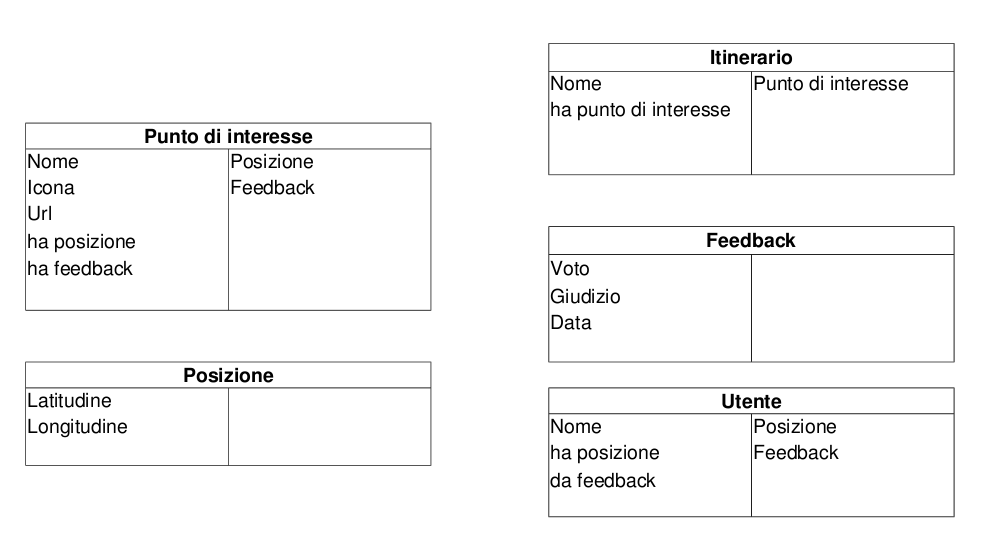
\includegraphics[scale=0.50]{imgs/model/crcmodel.png}
\caption{Modello CRC dell'applicazione\label{crcmodel}}
\end{center}
\end{figure}
Per modellare il dominio vengono qui utilizzate le \textit{Class Responsibility Collaborator (CRC) Cards}, come illustrato in figura \ref{crcmodel}.

\subsection{Modello dell'interfaccia utente}
L'interfaccia utente è la porzione di software che interagisce direttamente con l'utente.
In base ai requisiti non funzionali che caratterizzano l'interfaccia utente, si cerca di realizzare interfacce che tengano conto dell'usabilità.
Vengono riportati di seguito alcuni sketches che costituiscono le schermate dell'applicazione (fig. \ref{sketch}).
\begin{figure}[h!]
\subfloat[Home]{\label{mockuphome}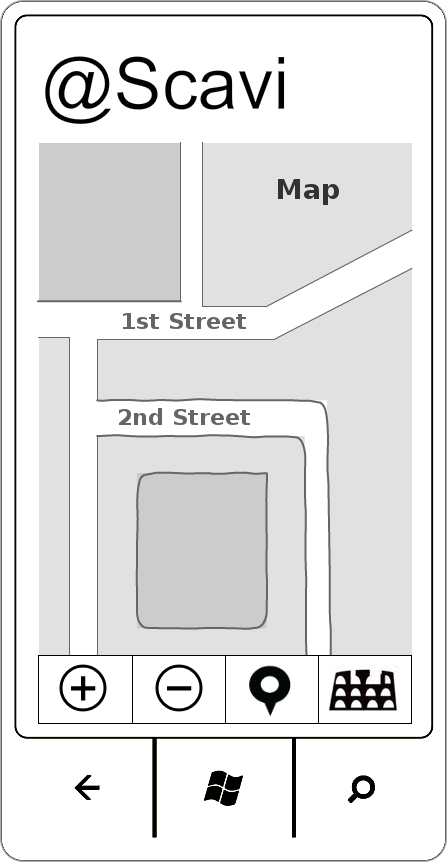
\includegraphics[scale=0.29]{imgs/mockup/home.png}}
\hspace{35mm}
\subfloat[Visualizzazione posizione]{\label{mockupposition}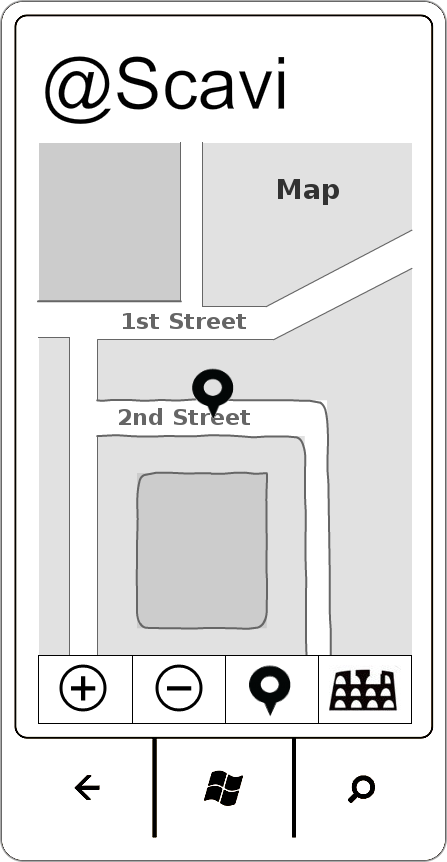
\includegraphics[scale=0.29]{imgs/mockup/position.png}}
 \hspace{35mm}
\subfloat[Visualizzazione punti di interesse]{\label{mockuppushpin}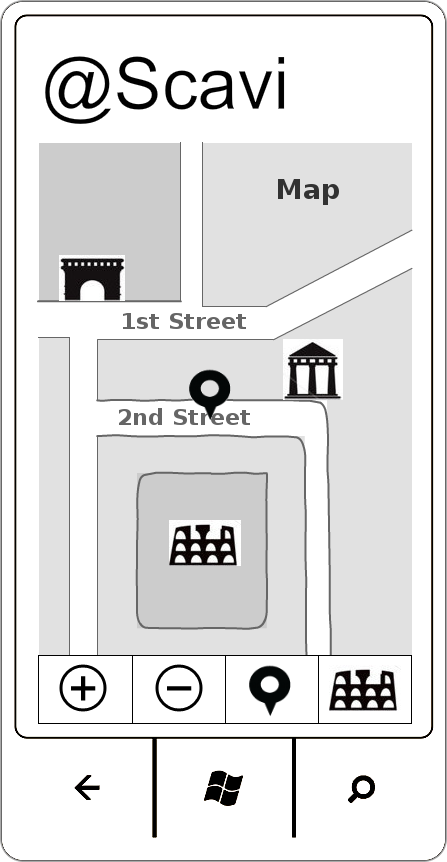
\includegraphics[scale=0.29]{imgs/mockup/pushpin.png}}
 \hspace{35mm}
\subfloat[Visualizzazione menu]{\label{mockuptooltipmenu}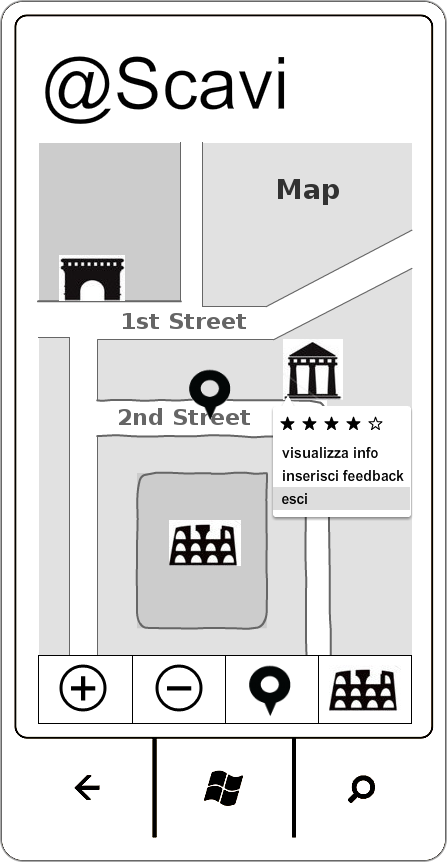
\includegraphics[scale=0.29]{imgs/mockup/tooltipmenu.png}} 
 \hspace{35mm}

\caption{Sketch dell'applicazione, 1\label{sketch}}
\end{figure}

\begin{figure}[h!]
\ContinuedFloat 
\subfloat[Visualizzazione dettaglio]{\label{mockupdetails}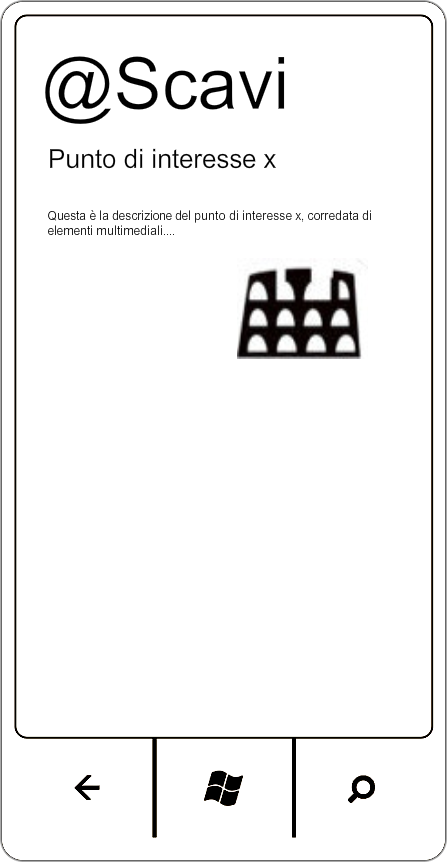
\includegraphics[scale=0.29]{imgs/mockup/details.png}}
 \hspace{35mm}
\subfloat[Invio feedback]{\label{mockupsendfeedback}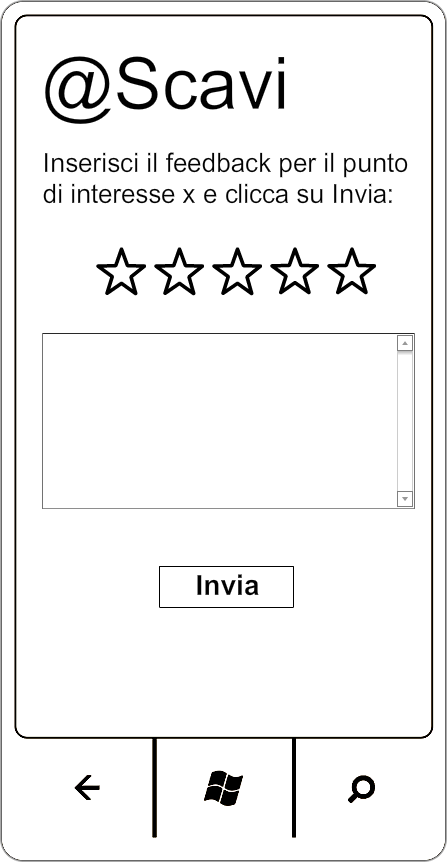
\includegraphics[scale=0.29]{imgs/mockup/sendfeedback.png}}
 \hspace{35mm}

\subfloat[Itinerario]{\label{mockupitinerario}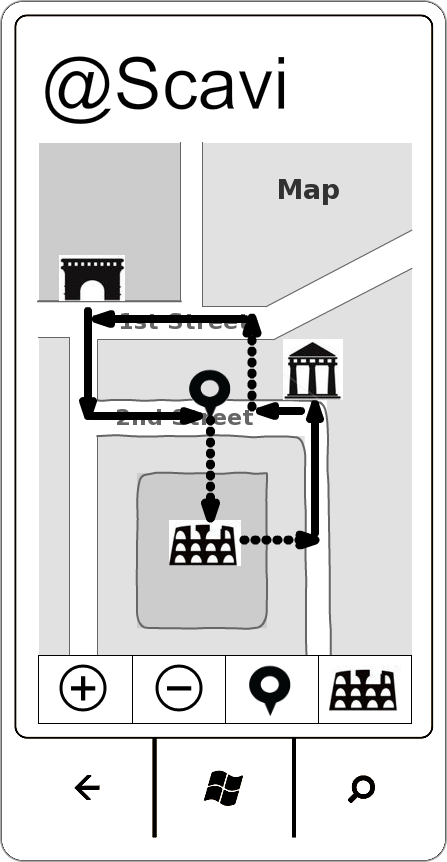
\includegraphics[scale=0.29]{imgs/mockup/route.png}}

\caption{Sketch dell'applicazione, 2\label{sketch}}
\end{figure}

%\Image[width=0.35\linewidth]{imgs/mockup/home.png}{Home}\,
%\Image[width=0.35\linewidth]{imgs/mockup/position.png}{Visualizzazione posizione}
%
%\Image[width=0.35\linewidth]{imgs/mockup/pushpin.png}{Visualizzazione punti di interesse}\,
%\Image[width=0.35\linewidth]{imgs/mockup/tooltipmenu.png}{Visualizzazione menu contestuale}
%
%\Image[width=0.35\linewidth]{imgs/mockup/details.png}{Visualizzazione dettagli} \,
%\Image[width=0.35\linewidth]{imgs/mockup/sendfeedback.png}{Invio feedback}
%
%\Image[width=0.35\linewidth]{imgs/mockup/route.png}{Itinerario}
%\captionof{figure}{Sketch dell'applicazione\label{sketch}}
\clearpage

\subsection{Pianificazione degli incrementi}
Tramite il planning poker\footnote{Il planning poker è una tecnica basata sul consenso per stimare lo sforzo nel completare una user story. E' largamente utilizzata in nelle metodologie agili.}, è stato possibile dare una stima della complessità delle user stories.

\begin{figure}[h!]
\begin{center}
\begin{tabular}[c]{|c|p{7cm}|c|c|}
\hline
N. & User story & Peso & Priorità\\
\hline
1 & \textit{essendo un utente vorrei poter visualizzare la mia posizione sulla mappa così da orientarmi meglio all'interno del sito} & 5 & 10\\
\hline
2 & \textit{essendo un utente vorrei poter visualizzare i punti di interesse sulla mappa così da spostarmi verso di essi} & 8 & 10\\
\hline
3 & \textit{essendo un utente vorrei poter zoomare e centrare la mappa così da ottenere una visualizzazione migliore} & 3 & 9\\
\hline
4 & \textit{essendo un utente vorrei poter sapere quando sono vicino ad un punto di interesse così da conoscere informazioni su di esso} & 5 & 8\\
\hline
5 & \textit{essendo un utente vorrei poter cliccare su un punto di interesse così da conoscere informazioni su di esso} & 3 & 7\\
\hline
6 & \textit{essendo un utente vorrei poter conoscere i feedback degli altri utenti così da spostarmi verso punti di interesse dal rating noto} & 3 & 6\\
\hline
7 & \textit{essendo un utente vorrei poter inviare un feedback così da condividere la mia esperienza con gli altri utenti} & 5 & 5\\
\hline
8 & \textit{essendo un utente vorrei poter ottenere un itinerario così da ottimizzare il tempo di visita} & 15 & 5\\
\hline
\end{tabular}
\caption{Tabella di stima delle user stories\label{userstoriestable}}
\end{center}
\end{figure}
\clearpage

In definitiva abbiamo la tabella in figura \ref{userstoriestable}, con stima e priorità delle user stories.
Considerando una velocità di 15 punti per iterazione e tenendo conto delle priorità, è stato possibile pianificare 3 iterazioni, ciascuna della durata di due settimane, come illustrato in figura \ref{pianificazioneiterazioni}.
Quindi, il progetto verrà sviluppato in sei settimane.
\begin{figure}[h!]
\begin{center}

\begin{tabular}[c]{|c|p{7cm}|c|c|}
\hline
Iterazione & User story\\ \hline
\textbf{Prima iterazione} & 1,2,3 \\ \hline
\textbf{Seconda iterazione} & 4,5,6,7\\ \hline
\textbf{Terza iterazione} & 8\\ \hline
\end{tabular}
\caption{Pianificazione delle iterazioni\label{pianificazioneiterazioni}}

\end{center}
\end{figure}

\clearpage

\section{Iterazione 1}
Nelle iterazione 1 viene effettuata l'analisi dei requisiti per tutti i requisiti corrispondenti alle user stories che ne fanno parte; vengono esplicitati i casi di test; vengono sviluppati alcuni modelli, in particolare i modelli strutturali (modello dei dati e diagramma delle classi) e i modelli comportamentali (diagramma di sequenza), migliorando e ridefinendo, se necessario, i modelli dell'iterazione precedente; vengono, inoltre, mostrati alcuni dettagli di implementazione corrispondenti a porzioni di codice; infine vengono mostrati gli screenshot dell'applicazione.\\

\subsection{Analisi dei Requisiti}
Nell'analisi dei requisiti, le \textit{user stories} vengono suddivise in task; i requisiti non funzionali vengono validati, migliorati e approfonditi.

%Gli sketch della prima iterazione sono quelli in figura \ref{sketch1iterazione}.
%\begin{figure}
%\subfigure[prima]{ 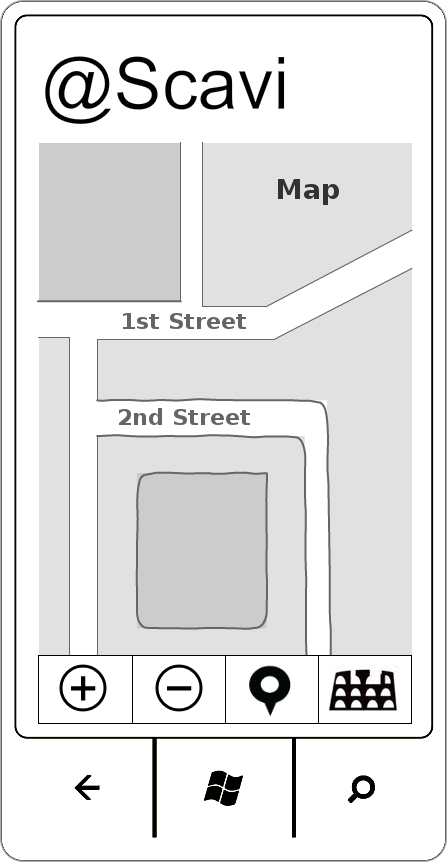
\includegraphics[scale=0.29]{imgs/mockup/home.png} }
%\subfigure[seconda]{ 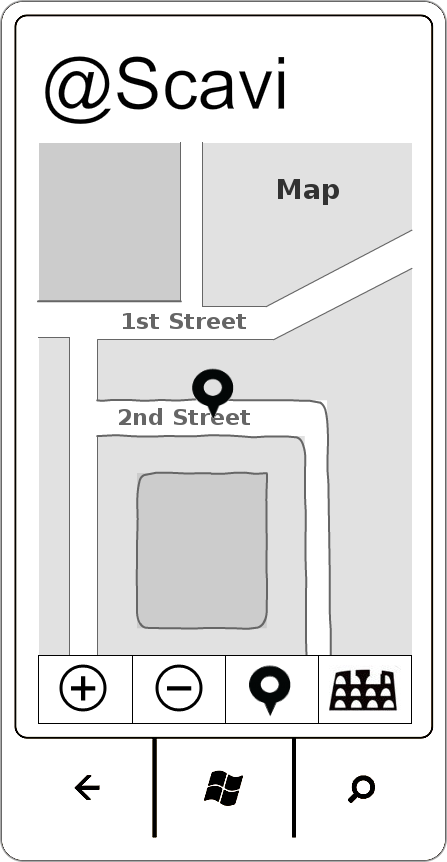
\includegraphics[scale=0.29]{imgs/mockup/position.png} }
%\subfigure[terza]{ 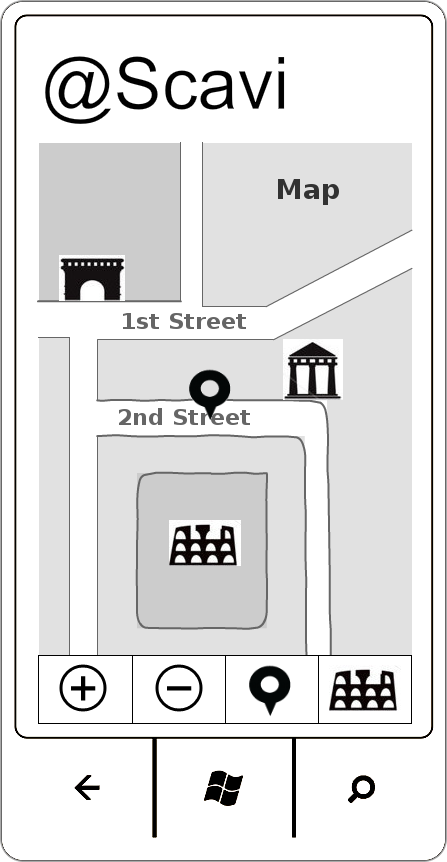
\includegraphics[scale=0.29]{imgs/mockup/pushpin.png} }
%\caption{Sketch della prima iterazione, I\label{sketch1iterazione}}
%\end{figure}
\subsubsection{Requisiti funzionali}
In questa iterazione, come già specificato prima, sono sviluppate le user stories 1,2 e 3 (fig. \ref{userstoriestableprimaiterazione}). \\
\begin{figure}[h!]
\begin{center}
\begin{tabular}[c]{|c|p{7cm}|c|c|}
\hline
N. & User story & Peso & Priorità\\
\hline
1 & \textit{essendo un utente vorrei poter visualizzare la mia posizione sulla mappa così da orientarmi meglio all'interno del sito} & 5 & 10\\
\hline
2 & \textit{essendo un utente vorrei poter visualizzare i punti di interesse sulla mappa così da spostarmi verso di essi} & 8 & 10\\
\hline
3 & \textit{essendo un utente vorrei poter zoomare e centrare la mappa così da ottenere una visualizzazione migliore} & 3 & 9\\
\hline
\end{tabular}
\caption{Tabella di stima delle user stories della prima iterazione\label{userstoriestableprimaiterazione}}
\end{center}
\end{figure}
\clearpage

Considerando le tre user stories, possiamo definire i seguenti task che caratterizzeranno la prima iterazione:\\
\textbf{Lato client}
\begin{itemize}
\item \textbf{creazione form con mappa e pulsanti di utility};
\item \textbf{visualizzazione posizione sulla mappa};
\item \textbf{visualizzazione punti di interesse sulla mappa};
\item \textbf{interfacciamento col dispositivo GPS};
\item \textbf{connessione al un servizio esterno};
\item \textbf{gestione dei layer della mappa}.
\end{itemize}

\textbf{Lato server}
\begin{itemize}
\item \textbf{mapping della base di dati};
\item \textbf{esportazione nel formato GeoRss}.
\end{itemize}

\subsubsection{Requisiti non funzionali}
I requisiti non funzionali già individati per questa prima iterazione sono presenti nella tabella in fig. \ref{nfrclient}.
Dopo un'analisi delle user stories e delle criticità presenti, possiamo individuare altri requisiti non funzionali:
\begin{itemize}
\item L'applicazione deve conservare i dati scaricati per la consultazione offline;
\item I punti di interesse devono avere icone diverse a seconda della tipologia;
\item La mappa deve essere centrata subito dopo la ricezione della posizione;
\item L'applicazione deve gestire l'assenza, la disattivazione e il mancato funzionamento delle periferiche GPS e di rete.
\end{itemize}

Per quanto riguarda il servizio, oltre ai requisiti già individuati nella tabella in fig. \ref{nfrserver}, definiamo il seguente requisito:
\begin{itemize}
\item Il servizio deve generare un file dal formato GeoRss conforme con gli standard di W3C.
\end{itemize}



\subsection{Casi di Test}
Durante l'analisi dei requisiti funzionali e non funzionali, è scaturito che particolare attenzione va posta, in questa fase, allo scambio dei dati col server ed alle periferiche di posizionamento e di rete.
Sono quindi sviluppati i seguenti test di accettazione:
\begin{enumerate}
\item Verificare l'avvio dell'applicazione.
\begin{enumerate}
\item Chiudere i dispositivi di rete o chiudere la connessione dati. \\Avviare l'applicazione. \\Verificare il messaggio di allerta che indica l'assenza di connessione dati e chiede di cliccare per aprire la form delle propietà di connessione.
\begin{enumerate}
\item Verificare la possibilità di chiudere il messaggio di allerta.
\item Verificare che cliccando si apra la form delle proprietà di connessione.
\item Verificare il reloading della schermata iniziale dell'applicazione con le nuove impostazioni.
\item Verificare il nuovo messaggio di alert nel caso non vi sia ancora connettività.
\end{enumerate}

\item Attivare i dispositivi di rete. \\Assicurarsi della presenza di una connessione dati attiva. \\Avviare l'applicazione. \\Verificare l'avvio della schermata principale con mappa e barra dei pulsanti di utility.
\begin{enumerate} 
\item Verificare la possibilità di cliccare e spostarsi sulla mappa.
\end{enumerate}
\end{enumerate}

\item Verificare il funzionamento del pulsante di posizionamento.
\begin{enumerate}
\item Spegnere il dispositivo di puntamento o assicurarsi di mancanza di ricezione del segnale GPS. \\Cliccare sul pulsante per ottenere la posizione attuale. \\Verificare il messaggio di allerta che indica l'assenza di dispositivi di posizionamento e chiede di cliccare per aprire la form delle propietà del GPS. 
\begin{enumerate}
\item Verificare la possibilità di chiudere il messaggio di allerta.
\item Verificare che cliccando si apra la form delle proprietà del posizionamento.
\item Nel caso siano stati attivati dispositivi di puntamento, verificare l'aggiornamento automatico della mappa alla posizione corrente.
\end{enumerate}
\item Attivare il dispositivo GPS e assicurarsi della ricezione del segnale GPS. \\Cliccare sul pulsante per ottenere la posizione attuale. \\Verificare che sulla mappa venga segnalata la posizione attuale.
\begin{enumerate}
\item Verificare che la mappa venga centrata sulla posizione attuale
\end{enumerate}
\end{enumerate}

\item Verificare il funzionamento del pulsante di visualizzazione dei punti di interesse.
\begin{enumerate}
\item Chiudere i dispositivi di rete o chiudere la connessione dati. \\Cliccare sul pulsante di visualizzazione dei punti di interesse.\\ Verificare il messaggio di allerta che indica l'assenza di connessione dati e chiede di cliccare per aprire la form delle propietà di connessione.
\begin{enumerate}
\item Verificare la possibilità di chiudere il messaggio di allerta.
\item Verificare che cliccando si apra la form delle proprietà di connessione.
\item Verificare il reloading della mappa con le nuove impostazioni e, nel caso vi sia connessione dati attiva, la visualizzazione dei punti di interesse.
\end{enumerate}

\item Attivare i dispositivi di rete. \\Assicurarsi della presenza di una connessione dati attiva. \\Cliccare sul pulsante di visualizzazione dei punti di interesse. \\Porre in ingresso uno stream di dati GeoRss valido.
\begin{enumerate}
\item Verificare visualizzazione punti di interesse sulla mappa
\end{enumerate}

\item Attivare i dispositivi di rete. \\Assicurarsi della presenza di una connessione dati attiva. \\Cliccare sul pulsante di visualizzazione dei punti di interesse. \\Porre in ingresso uno stream di dati GeoRss non valido, incompleto o nullo. \\Verificare il messaggio di allerta che indica l'errato parsing del file.
\begin{enumerate}
\item Verificare la possibilità di chiudere il messaggio di allerta.
\item Verificare il ritorno alla visualizzazione precedente.
\end{enumerate}
\item Attivare i dispositivi di rete.\\Assicurarsi della presenza di una connessione dati attiva.\\Cliccare sul pulsante di visualizzazione dei punti di interesse. \\Rendere inaccessibile il servizio per lo stream dei dati GeoRss.\\Verificare il messaggio di allerta che indica la mancata accessibilità del servizio.
\begin{enumerate}
\item Verificare la possibilità di chiudere il messaggio di allerta.
\item Verificare il ritorno alla visualizzazione precedente.
\end{enumerate}
\end{enumerate}
\item Cliccare sui pulsanti di zoom. \\Verificare l'ingrandimento o la riduzione della scala della mappa.
\end{enumerate}


\subsection{Modellazione}
\subsubsection{Modelli strutturali}
\paragraph{Modello dei dati}
\subparagraph{Client}
Nell'iterazione 1, il client gestisce tre tipologie di dati:
\begin{itemize}
\item \textbf{Punto di interesse}
\item \textbf{Tipologia}
\item \textbf{Posizione}
\end{itemize}
Per cui abbiamo un modello dei dati che può essere sintetizzato come in fig. \ref{datamodel1iterazione}.
\begin{figure}
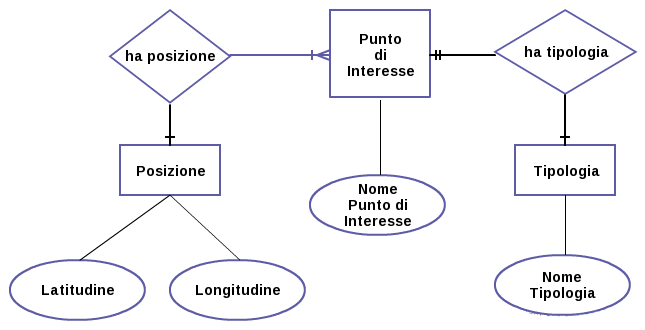
\includegraphics[scale=0.55]{imgs/model/DataModel1.png} 
\caption{Modello dei dati prima iterazione\label{datamodel1iterazione}}
\end{figure}

\paragraph{Diagramma delle classi}

\subsubsection{Modelli comportamentali}
\paragraph{Diagramma di sequenza}
\subsection{Implementazione}

\subsection{Screenshot}





\clearpage

\section{Iterazione 2}

\subsection{Analisi dei requisiti}

\subsubsection{Requisiti funzionali}
Nell'iterazione 2 sono sviluppate le user stories 4,5,6 e 7 (fig. \ref{userstoriestablesecondaiterazione}). 
\begin{figure}
\begin{center}
\begin{tabular}[c]{|c|p{7cm}|c|c|}
\hline
N. & User story & Peso & Priorità\\
\hline
4 & \textit{essendo un utente vorrei poter sapere quando sono vicino ad un punto di interesse per poter conoscere informazioni su di esso} & 5 & 8\\
\hline
5 & \textit{essendo un utente vorrei poter cliccare su un punto di interesse per poter conoscere informazioni su di esso} & 3 & 7\\
\hline
6 & \textit{essendo un utente vorrei poter conoscere i feedback degli altri utenti per poter spostarmi verso punti di interesse dal rating noto} & 3 & 6\\
\hline
7 & \textit{essendo un utente vorrei poter inviare un feedback per condividere la mia esperienza con gli altri utenti} & 5 & 5\\
\hline
\end{tabular}
\caption{Tabella di stima delle user stories della seconda iterazione\label{userstoriestablesecondaiterazione}}
\end{center}
\end{figure}

Considerando queste quattro user stories, possiamo definire i seguenti task che caratterizzano la seconda iterazione:\\
\textbf{Lato client}
\begin{itemize}
\item \textbf{realizzazione form per visualizzazione di informazioni sul punto di interesse};
\item \textbf{realizzazione servizio per la gestione della posizione sulla mappa};
\item \textbf{connessione al servizio di lettura feedback};
\item \textbf{menu contestuale con visualizzazione feedback};
\item \textbf{connessione al servizio di scrittura feedback};
\item \textbf{realizzazione form per inserimento feedback}.
\end{itemize}

\textbf{Lato server}
\begin{itemize}
\item \textbf{creazione servizio per la lettura dei feedback};
\item \textbf{creazione servizio per la scrittura dei feedback}.
\end{itemize}


\subsubsection{Requisiti non funzionali}
Oltre ai requisiti non funzionali già elencati, per l'applicazione si aggiungono i seguenti requisiti:
\begin{itemize}
\item L'applicazione deve gestire la situazione in cui la distanza da due o più punti di interesse sia uguale.
\item L'applicazione deve gestire localmente la vicinanza ai punti di interesse.
\item L'utente può inviare feedback anonimamente.
\item L'utente può inviare al massimo un feedback per ogni punto di interesse.
\item Il commento di feedback deve essere contenuto nei 1000 caratteri.
\end{itemize}

Per il server, invece si può aggiungere:
\begin{itemize}
\item Il sistema deve generare un codice hash per ogni utente.
\end{itemize}



\subsection{Casi di Test}
Dopo l'analisi dei requisiti funzionali e non funzionali, sono stati sviluppati i seguenti casi di test:
\begin{enumerate}
\item Verificare visualizzazione automatica informazioni sul punto di interesse
\begin{enumerate}
\item Assicurarsi che sulla mappa siano visibili i punti di interesse.\\
Assicurarsi della presenza del segnale GPS.\\
Assicurarsi della presenza di una connessione dati attiva.\\
Avvicinarsi fisicamente ad un punto di interesse.\\
\begin{enumerate}
\item Verificare la visualizzazione sul display di informazioni sul punto di interesse.
\item Verificare la possibilità di ritornare alla schermata precedente.
\end{enumerate}
\end{enumerate}
\item Verificare visualizzazione informazioni sul punto di interesse tramite click
\begin{enumerate}
\item Assicurarsi che sulla mappa siano visibili i punti di interesse.\\
Assicurarsi della presenza di una connessione dati attiva.\\
Cliccare sull'icona rappresentante il punto di interesse scelto.
\begin{enumerate}
\item Verificare la visualizzazione di un popup con una voce "visualizza info".
\item Verificare la possibilità di cliccare sulla voce "visualizza info".
\item Verificare la visualizzazione delle informazioni riguardanti il punto di interesse cliccato.
\item Verificare la possibilità di tornare alla schermata precedente.
\end{enumerate}
\end{enumerate}
\item Verificare visualizzazione feedback
\begin{enumerate}
\item Assicurarsi che sulla mappa siano visibili i punti di interesse.\\
Assicurarsi della presenza di una connessione dati attiva.\\
Cliccare sull'icona rappresentante il punto di interesse scelto.
\begin{enumerate}
\item Verificare la visualizzazione di un popup.
\item Verificare la presenza, nella parte superiore del popup, di cinque stelle, colorate a seconda del rating.
\item Verificare la possibilità di tornare alla schermata precedente.
\end{enumerate}
\end{enumerate}
\item Verificare invio feedback
\begin{enumerate}
\item Assicurarsi che sulla mappa siano visibili i punti di interesse.\\
Assicurarsi della presenza di una connessione dati attiva.\\
Cliccare sull'icona rappresentante il punto di interesse scelto.
\begin{enumerate}
\item Verificare la visualizzazione di un popup con una voce "inserisci feedback".
\item Verificare la possibilità di cliccare sulla voce "inserisci feedback".
\item Verificare la visualizzazione sul display di un form perd l'inserimento del feedback.
\item Verificare la possibilità di cliccare sul controllo contenete le cinque stelle.
\item Verificare la possibilità di inserire contenuti nella casella testo.
\item Verificare la possibilità di premere il pulsante "invia" per inviare il feedback.
\end{enumerate}
\end{enumerate}
\end{enumerate}


\subsection{Modellazione}
\subsubsection{Modelli strutturali}
\paragraph{Modello dei dati}
\subparagraph{Client}
Nell'iterazione 1, il client gestisce tre tipologie di dati:
\begin{itemize}
\item \textbf{Punto di interesse}
\item \textbf{Tipologia}
\item \textbf{Posizione}
\end{itemize}
Per cui abbiamo un modello dei dati che può essere sintetizzato come in fig. \ref{datamodel1iterazione}.
\begin{figure}
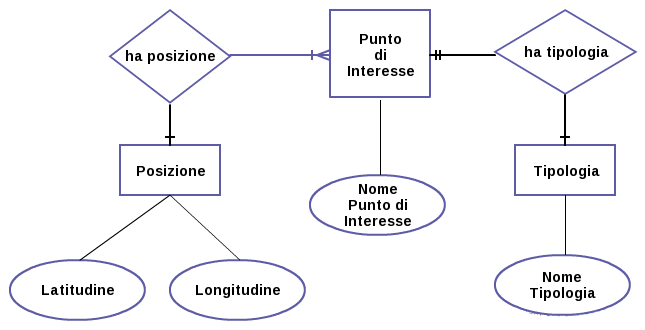
\includegraphics[scale=0.55]{imgs/model/DataModel1.png} 
\caption{Modello dei dati prima iterazione\label{datamodel1iterazione}}
\end{figure}

\paragraph{Diagramma delle classi}

\subsubsection{Modelli comportamentali}
\paragraph{Diagramma di sequenza}
\subsection{Implementazione}

\subsection{Screenshot}


\clearpage

\section{Iterazione 3}

\subsection{Analisi dei requisiti}
\subsubsection{Requisiti funzionali}
Nell'iterazione 3 è sviluppata la user story 8 (fig. \ref{userstoriestableterzaiterazione}). 
\begin{figure}[h!]
\begin{center}
\begin{tabular}[c]{|c|p{6cm}|c|c|}
\hline
N. & User story & Peso & Priorità\\
\hline
8 & \textit{essendo un utente vorrei poter ottenere un itinerario per poter ottimizzare il tempo di visita} & 15 & 5\\
\hline
\end{tabular}
\caption{Tabella di stima delle user stories della terza iterazione\label{userstoriestableterzaiterazione}}
\end{center}
\end{figure}

Considerando tale user story, possiamo definire i seguenti task che caratterizzano la terza iterazione:\\
\textbf{Lato client}
\begin{itemize}
\item \textbf{realizzazione form per visualizzazione dell'itinerario};
\item \textbf{connessione al servizio per la gestione della posizione}.
\end{itemize}

\textbf{Lato server}
\begin{itemize}
\item \textbf{realizzazione servizio per la gestione della posizione};
\item \textbf{realizzazione servizio per la creazione del feedback}.
\end{itemize}

\subsubsection{Requisiti non funzionali}
Oltre ai requisiti non funzionali già descritti nelle precedenti iterazioni, per le funzionalità previste in questa fase, si può aggiungere:
\begin{itemize}
\item L'itinerario deve tener conto della posizione dell'utente ed indicare la direzione
\item L'utente deve poter conoscere in ogni momento la distanza mancante alla fine dell'itinerario.
\end{itemize}

\subsection{Casi di Test}
\subsection{Modellazione}
\subsubsection{Modelli strutturali}
\paragraph{Modello dei dati}
\subparagraph{Client}
Nell'iterazione 1, il client gestisce tre tipologie di dati:
\begin{itemize}
\item \textbf{Punto di interesse}
\item \textbf{Tipologia}
\item \textbf{Posizione}
\end{itemize}
Per cui abbiamo un modello dei dati che può essere sintetizzato come in fig. \ref{datamodel1iterazione}.
\begin{figure}
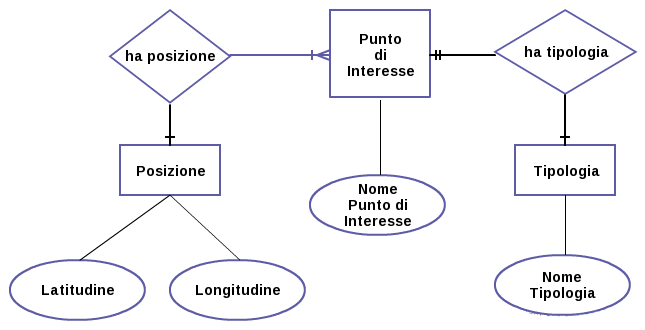
\includegraphics[scale=0.55]{imgs/model/DataModel1.png} 
\caption{Modello dei dati prima iterazione\label{datamodel1iterazione}}
\end{figure}

\paragraph{Diagramma delle classi}

\subsubsection{Modelli comportamentali}
\paragraph{Diagramma di sequenza}
\subsection{Implementazione}
\subsection{Screenshot}

\clearpage
%%%%%%%%%%%%%%%%%%%%%%%%%%%%%%%%%%%%%%%%%%%%%%%%%%%%%%

\clearpage{\pagestyle{empty}\cleardoublepage}